\documentclass[a4paper, 12pt]{article}

\usepackage[utf8]{inputenc}
\usepackage[T1]{fontenc}
\usepackage[english]{babel}
\usepackage{amsmath, amssymb}
\usepackage{graphicx}
\usepackage{hyperref}
\usepackage{float}
\usepackage{geometry}
\usepackage{fancyhdr}
\usepackage{caption}
\usepackage{graphicx}  % For images
\usepackage{hyperref}  % For hyperlinks
\usepackage{tikz}
\usepackage{capt-of}
\usepackage{listings}
\usepackage{xcolor}
\usepackage{sectsty}
\usepackage{sectsty}
\usepackage[scaled]{helvet}
\renewcommand{\familydefault}{\sfdefault}

\definecolor{darkblue}{RGB}{0,0,139}  % You can change the RGB if you want another shade
\sectionfont{\color{darkblue}}        % color for \section
\subsectionfont{\color{darkblue}}     % color for \subsection
\subsubsectionfont{\color{darkblue}}  % (optional) if you use subsubsections
\usepackage[utf8]{inputenc}  % Gestion UTF-8 (sous pdflatex)
\usepackage[T1]{fontenc}     % Encodage des fontes
\usepackage{amsmath}

\usetikzlibrary{arrows.meta, positioning}

% Marges
\geometry{margin=2.5cm}

% En-tête personnalisé
\pagestyle{fancy}
\fancyhf{}
\fancyhead[L]{Sorbonne Université}
\fancyhead[C]{Cubesat Attitude determination}
\fancyhead[R]{Faculty of Engineering}
\fancyfoot[C]{\thepage}

\lstset{
  language=Matlab,
  basicstyle=\ttfamily\small,
  keywordstyle=\color{blue}\bfseries,
  commentstyle=\color{green!50!black}\itshape,
  stringstyle=\color{red},
  numbers=left,
  numberstyle=\tiny\color{gray},
  stepnumber=1,
  breaklines=true,
  showstringspaces=false,
  frame=single,
  inputencoding=utf8
}


% Début du document
\begin{document}

% Page de garde
\begin{titlepage}
    \vspace*{\fill}  % Push content to the middle vertically
    \centering

    \begin{minipage}{0.45\textwidth}
        \centering
        
\includegraphics[width=0.6\textwidth]{fig/SU.jpg}
    \end{minipage}%
    \hfill
    \begin{minipage}{0.45\textwidth}
        \centering
        
\includegraphics[width=0.8\textwidth]{fig/Academie_Spatiale.png}
    \end{minipage}

    \vspace{5cm}

    {\bfseries\Huge Low-Cost Cubesat Attitude Determination\par}
\vspace{0.9cm}
{\bfseries\Huge Datasheet\par}
        \vspace{3cm}
    \textsc{\LARGE Sorbonne Université}\\[1cm]
    \textsc{\Large Académie Spatiale d'ile de France }\\[1cm]
    \textsc{\Large France 2030 }\\[1cm]
    \vspace{3cm}
    \textbf{Date: \today}

    \vspace*{\fill}  % Push bottom content to the bottom so that center aligns
\end{titlepage}

\newpage
\tableofcontents
\newpage
\listoffigures
\newpage

\section{Introduction}
\subsection{Project Overview}
This project focuses on the development of an attitude determination system for a CubeSat operating in low Earth orbit. The system utilizes data from an onboard magnetometer and a sun sensor (6 Solar panels), to estimate the satellite’s orientation relative to the Earth. The core processing and control algorithms are implemented on an ESP32 microcontroller, enabling real-time sensor data acquisition, processing, and attitude estimation.

\section{Applications}
The system is designed for low-budget missions (e.g., university projects, academic missions, research laboratories).

\section{Project Scope}
\begin{itemize}
    \item Designing and simulating an attitude determination system using magnetometer and sun sensor data
    \item Validating the system using test data
    \item Hardware implementation
    \item Documenting the methodology, results, and potential improvements
    \item Providing recommendations for future hardware implementation and integration
\end{itemize}

\newpage
\section{System Design}
\subsection{Overall Architecture}
\begin{figure}[H]  % Use [H] to place exactly here (requires the float package)
    \centering
    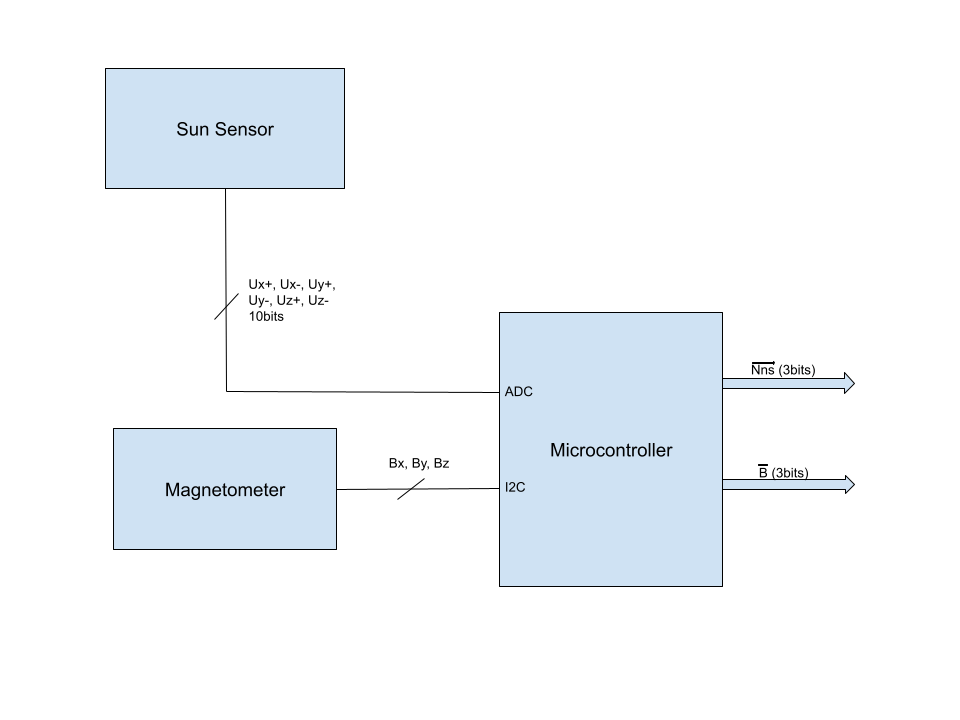
\includegraphics[width=0.9\textwidth]{fig/Architecture_globale.png}
    \caption{System architecture}
    \label{fig:System architecture}
\end{figure}


\subsection{System Schematic}
\begin{figure}[H]  % Use [H] to place exactly here (requires the float package)
    \centering
    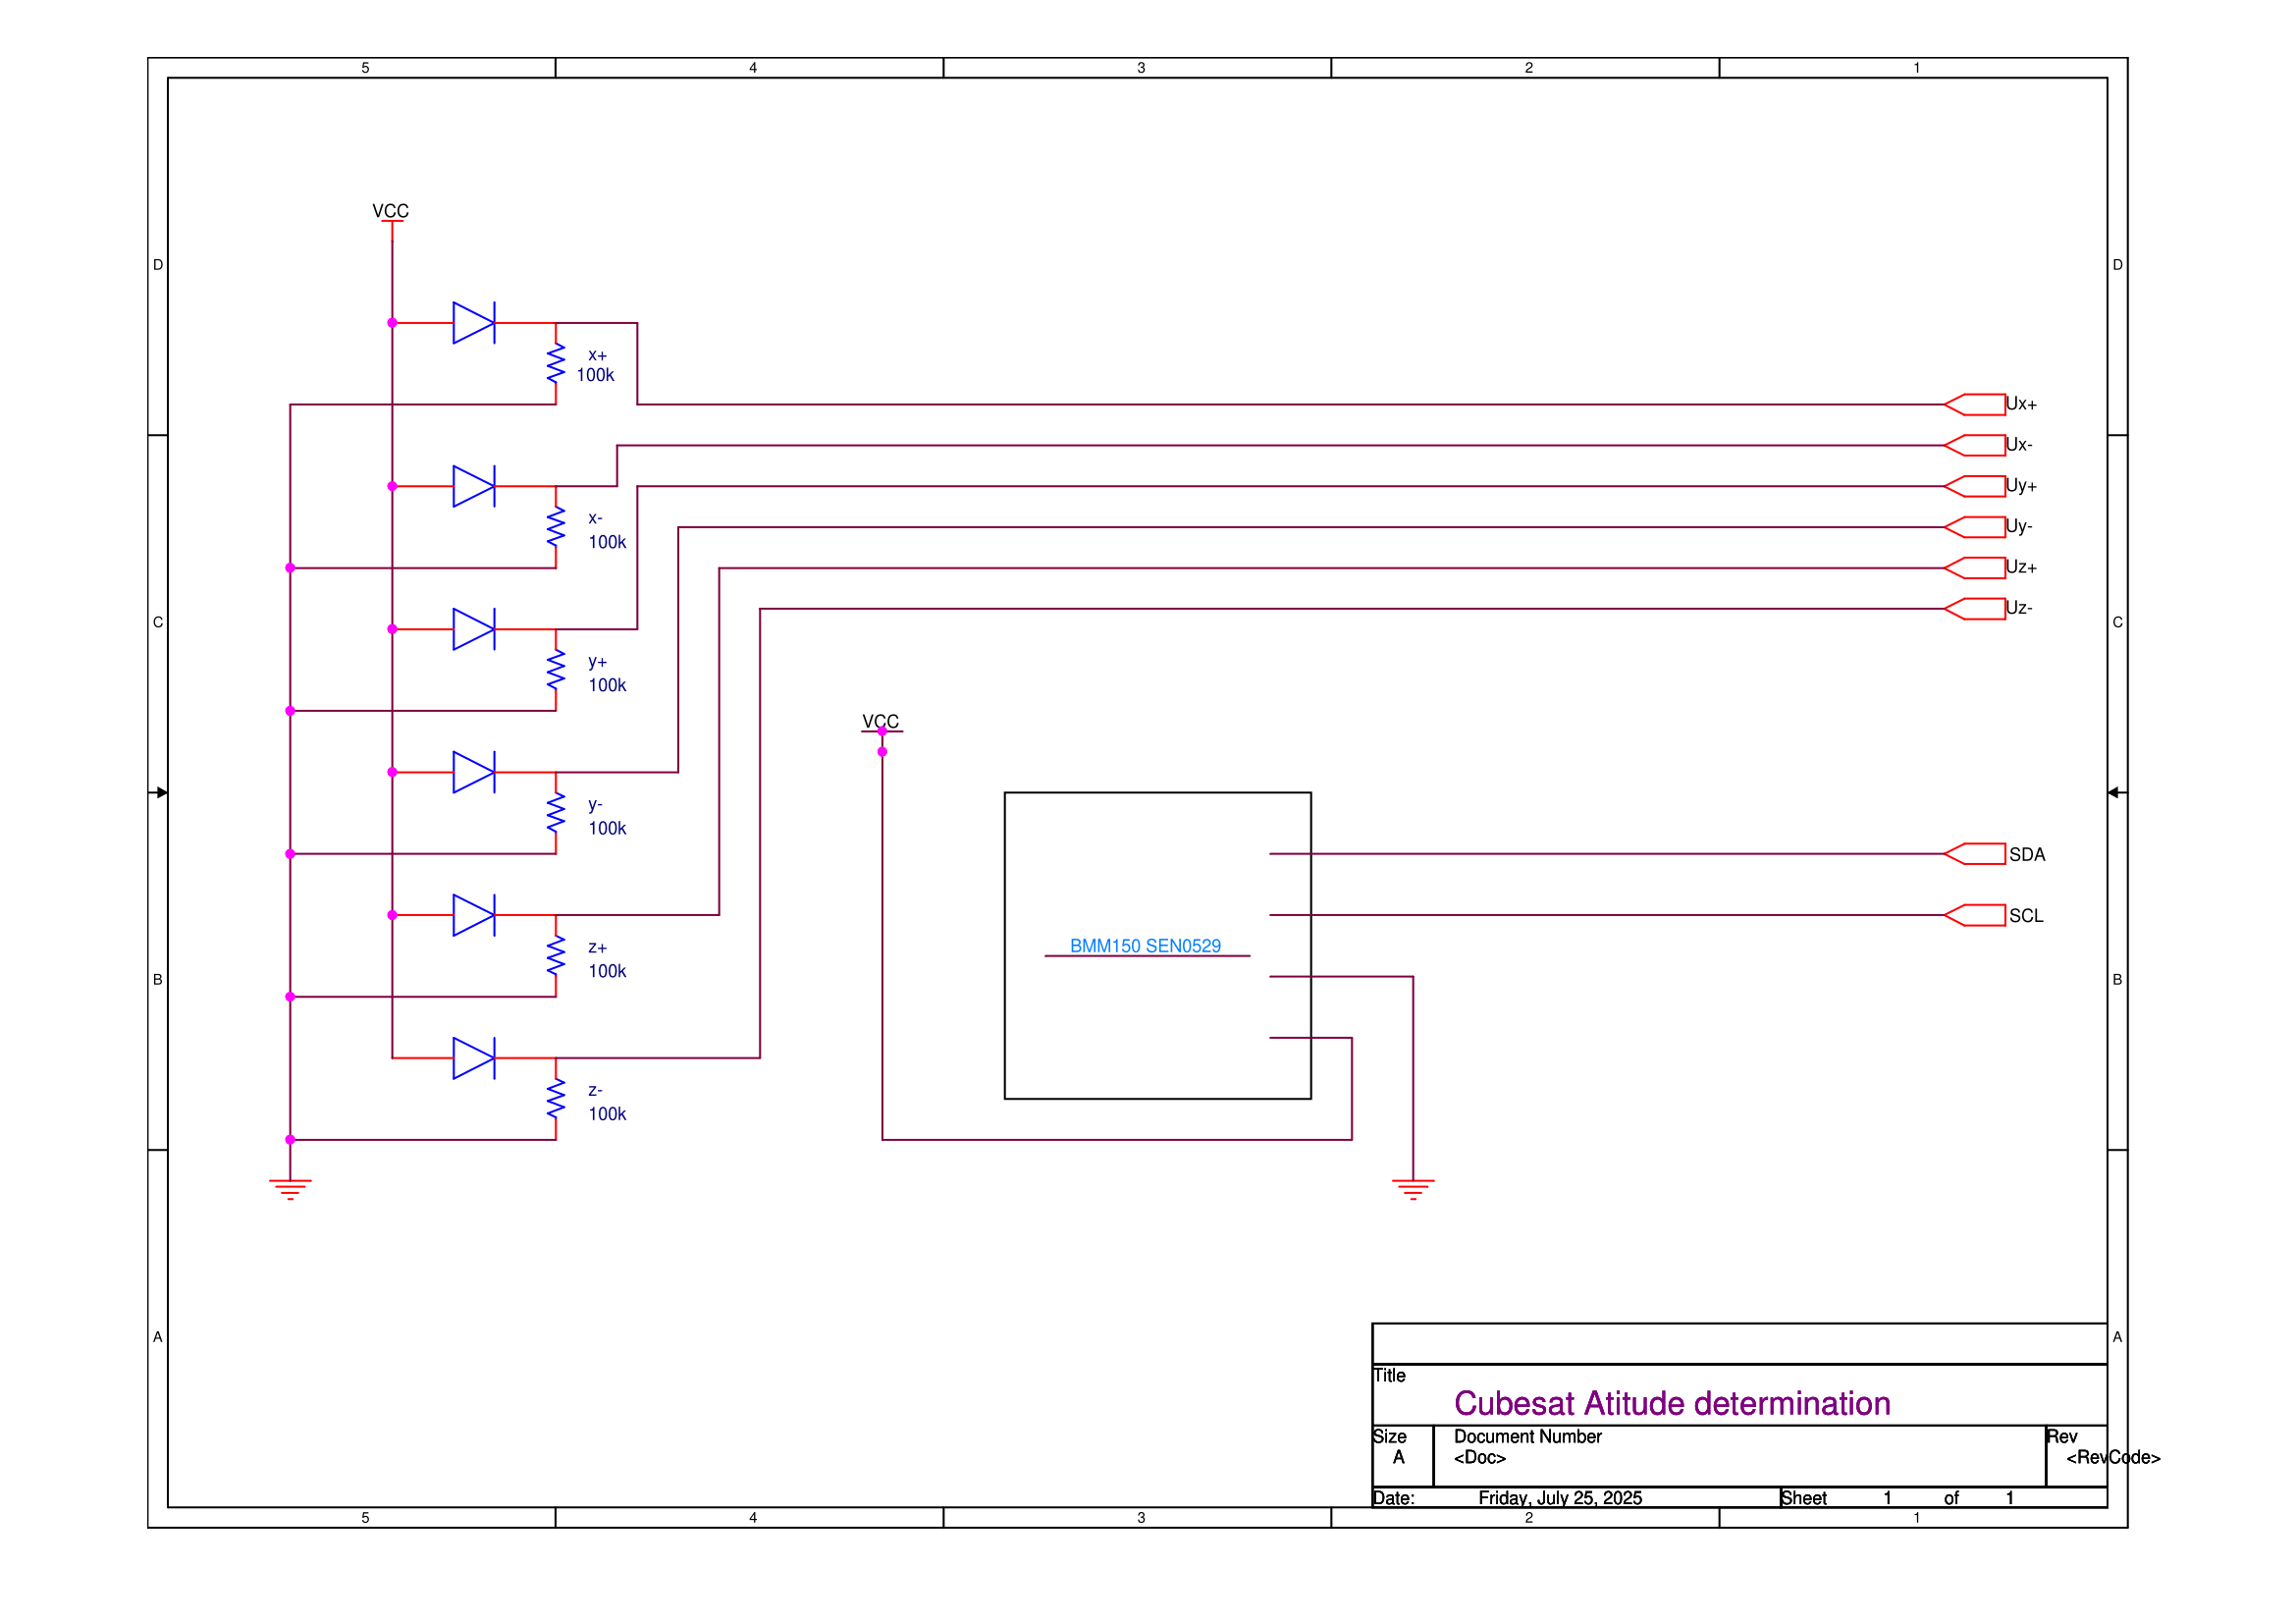
\includegraphics[width=1\textwidth]{fig/cubesatSchematic.png}
    \caption{System Schematic}
    \label{fig:System Schematic}
\end{figure}


\subsection{Hardware}

\begin{minipage}{0.55\textwidth}
\textbf{Solar Panel} 

The main function of the solar panel is to acquire data about the light intensity on each side of the CubeSat in order to calculate the sun-satellite vector.

\end{minipage}
\hfill
\begin{minipage}{0.4\textwidth}
    \centering
    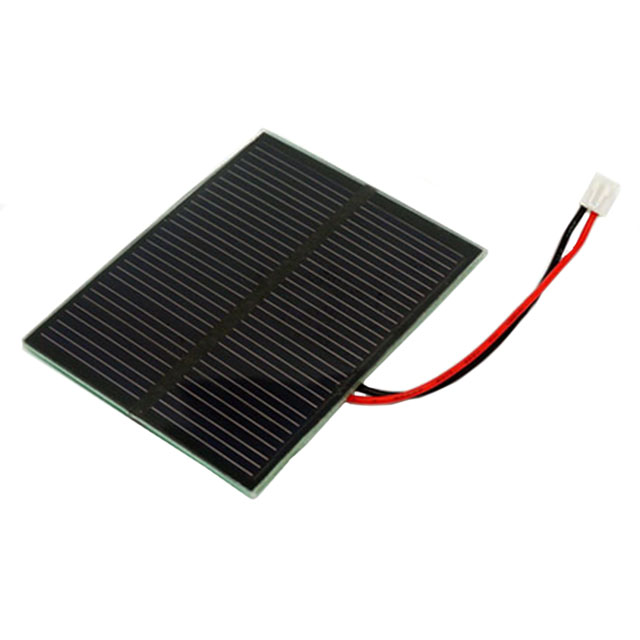
\includegraphics[width=0.5\linewidth]{fig/solarPanel.jpg}
    \captionof{figure}{Solar Panel 0.5W}
    \label{fig:Solar Panel}
\end{minipage}
\begin{minipage}{0.55\textwidth}
\textbf{Magnetometer} 

The magnetometer's role is to measure the magnetic field vector in the satellite's frame.

\end{minipage}
\hfill
\begin{minipage}{0.4\textwidth}
    \centering
    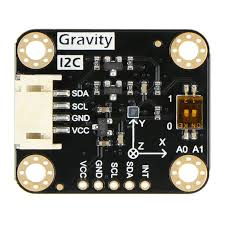
\includegraphics[width=0.5\linewidth]{fig/magnetometer.jpeg}
    \captionof{figure}{Magnetometer 3 axis BMM150 SEN0529}
    \label{fig:Magnetometer}
\end{minipage}
\begin{minipage}{0.55\textwidth}
\textbf{Microcontroller} 

The microcontroller combines the data issued from the two sensors in order to determine the attitude of the CubeSat.

\end{minipage}
\hfill
\begin{minipage}{0.4\textwidth}
    \centering
    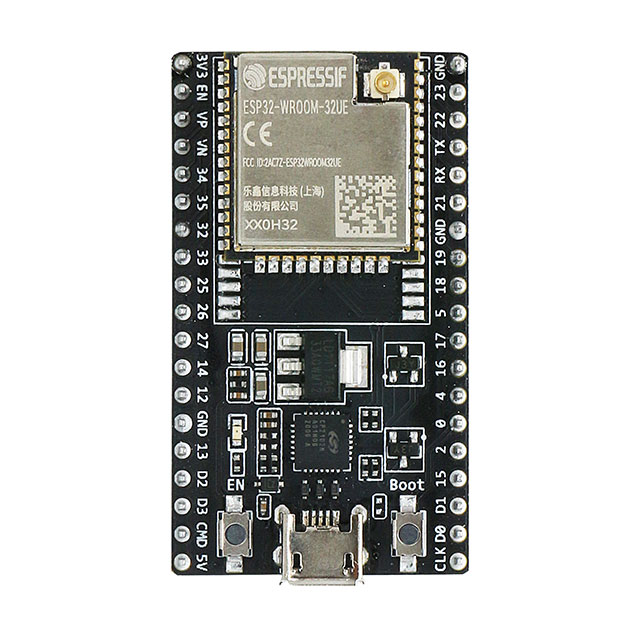
\includegraphics[width=0.5\linewidth]{fig/ESP32.jpg}
    \captionof{figure}{Microcontroller ESP32}
    \label{fig:Microcontroller}
\end{minipage}

\subsection{Software}

\end{document}